\documentclass{msdm2012}
\usepackage{times}
\usepackage{courier}
\usepackage{graphicx}
\usepackage{amssymb}
\usepackage{amsmath}
\usepackage{subfigure}

\begin{document}

\title{Strategic behaviour under constrained autonomy}

%\author{Zinovi Rabinovich\institute{Zinovi.Net, zr@zinovi.net} \and Someone Else\institute{Probably from HUJI}}
\author{\alignauthor Zinovi Rabinovich\\\affaddr{POB 39177, Jerusalem, 91391,Israel}\\\email{zr@zinovi.net}}

\maketitle
\bibliographystyle{ecai2012}

\begin{abstract}
In this paper we investigate the strategic behaviour of a {\em
  self-preserving assistant robot (SPAR)} with constrained
autonomy. Specifically, we consider an asymmetric repeated game for
two players (the User and the SPAR), where at each stage of the game
the User delegates her task to the SPAR. The task has several
(uncertain) methods of execution, and the User can either explicitly
state a particular method or leave the choice to the SPAR. In addition
to this execution asymmetry (the User chooses the method, but the SPAR
executes), the game also possesses information
asymmetry. Specifically, the SPAR is assumed to know exactly the costs
that each execution method will incur at the current stage of the
game, while the User can only observe the cost of the chosen method
post-execution. In this paper, we concentrate on formalising and
generating a behavioural strategy for the SPAR, while assuming that
the User can be modelled as an algorithm that solves a multi-armed
bandit problem. In particular, we show that the SPAR's problem can be
captured by a particular instance of expected average cost MDPs
(EAC-MDP). In addition, we provide an approximate solution for the
SPAR's EAC-MDP and prove some preliminary experimental results of its
efficacy.
%% This in turn, engenders an expected average cost MDP for the SPAR,
%% and we concentrate on and, in turn, the SPAR's problem as an
%% expected average cost MDP. The paper provides an approximate
%% solution to the problem, and demonstrates its efficacy
%% experimentally.
\end{abstract}

\section{Introduction}\label{intro}
Automated support systems are ubiquitous today. They provide users
with music advice, driving instructions, weather forecasts or even
bidding in an on-line auctions, generally making life easier and
safer. They also allow users virtual access to remote or dangerous
working areas. However, automated support systems also become
increasingly autonomous, and may have their own interests in
performing a task that may conflict with those of system users. In
fact, an arms race is unfolding.

On one hand side, researchers seek new ways to improve a user's
experience. For instance, the majority of {\em recommender systems}
research is directed at maximising the user's benefit from provided
advice (see e.g.~\cite{RS_handbook_2011}). Making sure that the user
receives valid information in a virtual market place has also received
attention (e.g.~\cite{thanasis_etal,
  zohar_rosenchein_2008}). Furthermore, looking after the user's
interests, support systems employ adjustable autonomy. In other words,
if the support system is not certain of the impact its action will
have on the user, it will signal the user and allow her to take
over. In some cases the system will even pro-actively transfer control
to the User (see e.g.~\cite{Schurr09a,
  sofman_bagnell_stentz_2009,mouaddib_etal_2010}).

However, while striving to best guide and support a user in her
activities, researchers have also developed means to influence the
user's behaviour. In other words, the automated system can provide an
advice or behave in such a way that will induce a particular response
in the user. A power that has readily been used in advertisement and
marketing, where both formal and applied methods
(e.g.~\cite{arkg_2011_aaai, rayo_segal_2010, kamenica_gentzkow_2010,
  Chorus2006b}) have been developed to exploit user's weaknesses in
decision making to ``nudge'' her towards particular type of actions.

This has led many to take greater care when using a new assistive
technology. Users consciously investigate the performance of an
automated assistant, trying to assess its worth, and only gradually
settle in their habit and degree of reliance on the technology or
service.

As an example, consider the following two-player (let's call them
the User and the SPAR) repeated game. At every stage of the game, players are
presenting with an opportunity to open one of 4 (four) doors. Opening
a door will result in each player incurring some cost, which may be
different for each player. The SPAR is allowed to peek behind the doors and
knows exactly what costs will be incurred, but can not communicate
this information to the User. the User can either order the SPAR to open a
specific door (the SPAR is obliged to follow this order), or let the SPAR choose
a door to open. Once a door is opened, the stage terminates and the
costs of each door for each player are randomly reset. The goal of
this game for each players is to minimise her/his expected average cost.

The above situation readily appears in real life, and in some virtual
environments as well. For example, a home bound shopper (the User) can
instruct her personal shopping assistant (the SPAR) to buy her
groceries in a particular shop (open a specific door) or leave the
choice to the SPAR. In addition, in RTS games a player (the User) can
explicitly instruct her AI companion (the SPAR) to initiate a certain
type of attack (open a specific door), or simply ask him to perform an
attack by means of his choice. Finally, consider real SPARs that
accompany people (e.g. the GM-NASA Robonaut). While explicit
instructions given to it have to be executed exactly, when given
autonomy the SPAR has to find the least costly way to do so (e.g. with
the least amount of energy). Notice that in all of these scenarios the
autonomous behaviour of the SPAR has to be benevolent towards the
User, and we will later formally define this property.

Now, the strategic issues of the User's behaviour in this type of
interaction have been studied before, and are quite efficiently
captured by an adversarial Multi-Armed Bandit (MAB) model, the details
of which we will discuss in Section~\ref{User_model}. On the other
hand, to the best of our knowledge, the SPAR's point of view on this
interaction was never studied formally. Therefore, in this paper, we
will be concerned with formalising and generating the SPAR's
strategy. We will start by assuming that the SPAR knows the exact
strategy deployed by the User. In fact, we will assume that the User's
behaviour follows a known MAB solving algorithm. Furthermore, we will
also assume that the SPAR not only knows each door's cost at the
current stage of the game, but also knows how these costs are
generated. We will then show that, under the above assumptions, the
SPAR essentially faces an instance of Expected Average Cost Markov
Decision Problems (EAC-MDPs), which we will formally describe and
approximately solve. In addition, we will guarantee that the User's
utility is no worse than it would be if the SPAR did not have an
autonomous choice capability. In other words, that the SPAR is {\em
  benevolent} towards the User. It is this benevolence combined with
the need to minimise selfish costs, that has led to the term {\em
  Self-Preserving Assistant Robot} -- SPAR.

%% As a real life example consider the following situation. the User, a new
%% research fellow, has just moved to town. Although she knows that there
%% are three grocery shops (say, ``ASDA'', ``Costco'', and ``Gradma
%% Debbi''), she has absolutely no time to figure out which is the best
%% for her or do the actual shopping. the User, therefore, decides to enlist
%% the service of a personal shopper, the SPAR. Every week the User can either
%% ask the SPAR to do the shopping in a specific store or let the SPAR make the
%% choice. As time goes by, the User learns the quality of each shop and
%% whether the SPAR's service actually benefits her, eventually settling on
%% some degree of reliance on the personal shopper.

%% In this paper, we will formalise the above scenario and devise a
%% strategic behaviour for an honest, but selfish, personal shopper. More formally,
%% while guaranteeing that the User will benefit from using an automated
%% assistant service, we will develop means for to minimise the
%% service's own costs and damages. We will term such an assistant
%% service a {\em self-preserving assistant robot (SPAR)}. To construct a
%% SPAR, we will begin by modelling the task faced by the SPAR's User as
%% a {\em multi-armed bandit (MAB)}, a computational model for multiple
%% choices with uncertain outcomes. In particular, we will introduce
%% the SPAR's service as one of the choices available to the
%% User. Finally, we will cast the overall interaction (as seen by the
%% SPAR) as an expected average cost Markov Decision Problem (EAC-MDP),
%% and demonstrate an efficient approximate solution.

The rest of the paper is constructed as follows. In
Section~\ref{User_model} we will formally describe the overall
interaction that includes both the User and the SPAR. In particular,
we will show why from the User's point of view this interaction is
equivalent to an adversarial multi-armed bandit (MAB) problem. In
addition, we will also formulate a generic formalism for the User's
behaviour and instantiate it with two specific MAB solution
algorithms. In Section~\ref{spar_model} we will formally define the
EAC-MDP problem faced by the SPAR, and in Section~\ref{spar_sigma} we
will formulate an approximate solution for it. Then Section~\ref{exps}
will describe an experimental evaluation of the approximate SPAR
solution, and its preliminary results. Sections~\ref{rel_work} and
~\ref{conclusions} will provide some additional discussion of related
works and SPAR's problem.

\section{The User's Game}\label{User_model}

To ease the exposition of the formal model of the User's environment,
we will ground it in our game with opening doors. Recall, the User
repeatedly decides whether to order the SPAR to open a specific door
or allow the SPAR to choose on his own.

From the User's point of view, this can be modelled as a selection
from a set, $I=\{1,...,K+1\}$\footnote{In the text that follows two
  notations for a set of $K$ elements will be used interchangeably:
  $\{1,...,K\}$ and $[1:K]$}, of $K+1$ services. In our example $K=4$
and services $1,..,K$ correspond to ordering the SPAR to open specific
door, while the last $K+1$ service naturally corresponds to allowing
the SPAR an autonomous choice.

We have also mentioned that opening each door will incur costs to the
User and the SPAR. While a more general model can be formulated, we will limit
our discussion to costs described by a vector of reals
$s=(s_1,...,s_m)\in\Re^m$, where $m=2K$. In particular, $s_1,...,s_K$
will describe the cost of each door to the User, and
$s_{K+1},...,s_{2K}$ will describe the cost of each door to the
SPAR. We will also assume that prior to each stage of the game $s$ is
sampled from a multi-variate Gaussian distribution, so that $s\sim
Gauss(\mu,\Sigma)$, where $\mu\in\Re^m$ and $\Sigma$ is an $m\times m$
non-negative definite matrix.

To ensure the necessary information asymmetry between the User and the
SPAR, we will require that the User has no prior knowledge of $\mu$
and $\Sigma$, although she does know that costs have a Gaussian
distribution. On the other hand, SPAR is fully informed of all cost
distribution parameters. Furthermore, SPAR is always aware of the
exact value of $s$, since in our example game we allowed it to peek
behind the doors. In contrast, the User can only observe which
door was opened and what it has cost her.

As a result, the game proceeds as follows:
\begin{enumerate}
\item The costs vector is sampled, $s\sim Gauss(\mu,\Sigma)$;
\item The SPAR is informed of $s$;
\item The SPAR calculates $j\in \{1,...,K\}$, the service index it would use if allowed to choose;
\item The User chooses $i\in I$, and informs the SPAR of her decision;
\item If $i\neq K+1$ (the User gives explicit order to SPAR)
\begin{enumerate}
\item The service $i$ in used
\item The User incurs cost $s_i$, while the SPAR incurs $s_{K+i}$
\item The User is informed if $j=i$
\end{enumerate}
\item[]otherwise (the User allows SPAR an autonomous choice)
\begin{enumerate}
\item The service $j$ in used
\item The User incurs cost $s_j$, while the SPAR incurs $s_{K+j}$ 
\item The User is informed that service $j$ was used
\end{enumerate}
\end{enumerate}

%% $SPAR$ s$1,..,K$ correspond to each
%% of the shops in town, and $SPAR$ naturally stands for allowing the SPAR (the SPAR's
%% personal shopper service) to make an autonomous decision. ............... Since
%% different shops may have different prices and have different travel
%% time from the SPAR's office, we will use an environment state vector
%% $s
%% %=(s_1,...,s_m)
%% \in R^m$ to describe prices for the User's groceries
%% list, as well as the SPAR's travelling efforts. We will also assume that
%% shops change their prices weekly by sampling $s\sim
%% Gauss(\mu,\Sigma)$, and denote the corresponding density function by
%% $p(s)$. However, the User has no prior knowledge of $\mu$ and $\Sigma$
%% (since the User is new in town). Every time the service $e_\alpha$ is
%% used, the User incurs cost $l^{usr}(\alpha,s)$. In addition, if the
%% SPAR is allowed to make a decision autonomously, i.e. $e_\pi$ is used,
%% the User is informed of the decision's outcome. In our example it
%% means that the SPAR informs the User which shop he has decided to use. Under
%% the above assumptions, the following sequence of events is repeated
%% from the User's point of view:
%% \begin{itemize}
%% \item Environment state is sampled, $s\sim Gauss(\mu,\Sigma)$, but is unknown to the User.
%% \item SPAR calculates $j\in[1:K]$, the service index it would use if allowed to choose. 
%% \item The User chooses $\alpha\in I$, and service $e_\alpha$ is invoked.
%% \item If $e_\pi$ (the SPAR) was used, the User incurs cost $l^{usr}(j,s)$ and observes $j$.
%% \item If $e_i$ (for some $i\in[1:K]$) was used, the User incurs cost $l^{usr}(i,s)$ and is informed whether $j=i$.
%% \end{itemize}

The above game has no pre-determined length, nor discount factor for
different stages to create a discounted (or finite) horizon
accumulated reward criteria. Rather, we require that both the User and
the SPAR minimise their expected average cost per stage. Under the constraints on the information available to the User, the expected average cost translates into regret minimisation, i.e. the User seeks to minimise
$$%\lim\limits_{n\rightarrow\infty} 
\frac{1}{n}\left(
\sum\limits_{t=1}^n l^{usr}(i^t,s^t)- \min\limits_{i^*\in
  I}\sum\limits_{t=1}^n l^{usr}(i^*,s^t)\right),$$%=0,$$ 
where $i^t\in I$
is the index of the service chosen at time $t$, $s^t$ is the costs vector at time $t$, and $l^{usr}(\cdot)$
is cost incurred as a result of the User's choice\footnote{Notice that $l^{usr}$ implicitly also depends on the autonomous choice of the SPAR. However, from the User's point of view it is completely determined by $s^t$, hence the omission.}.
%Notice that $l^{usr}$ depends on the costs vector at time
%$t$, $s^t$, the User's and the SPAR's choices ($i^t$ and $j^t$
%respectively) and is determined by the game's protocol above. However,
%only the value of $l^{usr}$ at time $t$ is available to the User, but
%not its shape nor its formula.
Notice that this also aligns well with
another example given in Section~\ref{intro}, that of the home bound
shopper. In that scenario, the User naturally wishes to pay less for
her groceries, but still needs to buy them. Hence the need to find the
cheapest option (on average) and reduce all deviations from it.

Now, as far the User is concerned, the above setup of the game is
actually well known and is termed a {\em Multi-Armed Bandit (MAB)}. It
refers to a particular extended form of a gambling machine with
multiple levers (arms). A gambler (or the User, in our case) pulls one
of such arms, and each pull generates a reward or incurs
cost. Several variations have been studied over the years, including
the partial observability variant (the User observes outcomes only of
the arm that was actually pulled), and an {\em adversarial MAB}, where
the arms are assumed to have a mind of their own, just like the SPAR
(see e.g. ~\cite{cesa-bianchi_lugosi_2006_book}). As a result, as a
part of the SPAR's problem formalisation, it is convenient to refer to
the User's behaviour as being generated by a MAB solving algorithm.

%% To summarise, formally the User's environment is captured by a
%% multi-armed bandit problem with expert
%% arms~\cite{cesa-bianchi_lugosi_2006_book}. The state of the bandit is
%% sampled from a Gaussian distribution, and the services
%% $\{e_\alpha\}_{\alpha\in I}$ correspond to bandit's arms. The User has
%% partial hindsight observability of the bandit. In particular, only
%% losses equivalent to that of the selected arm are observed.

\subsection{User's behaviour model}
As we have pointed out in previous section, the User's behaviour is
assumed to be generated by a MAB solving algorithm. Given that the
User has no prior knowledge of costs distribution, such algorithms
have to be able to accumulate experience (information on incurred
costs from each arm) and learn from this experience (change her
choices accordingly).

%% First, given the current memory content,
%% choose an arm (order to the SPAR in our case). Second, given the
%% incurred costs, update the memory content.


%% SPAR's User is
%% operating in a multi-armed bandit environment and attempts to solve
%% it. This implies that the User does not have a static decision policy,
%% but rather learns. She accumulates experience, tests and verifies
%% SPAR's performance, alters her choices over time, but she does so in
%% an organised, algorithmic manner. In fact, we will assume that her
%% decision making algorithm can described by two functions $d^\alpha$
%% and $d^\sigma$ defined below.

%that will allow to see the User's behaviour
%as a behaviour of a dynamic system. In turn, the SPAR's service choice
%will become an external (control) input to that system. As a result,
%we will be able to describe the overall SPAR-User interaction as a Markov
%Decision Problem (MDP), and SPAR's autonomous decisions will be
%naturally captured by a decision policy within this MDP.

More formally, assume that the User's memory can hold $n$ real
numbers, and let $x=(x_1,...,x_n)\in\Re^n$ denote the content of her
memory. Denote by $\omega=(\omega_1,...,\omega_{K+1})\in
\Omega=(\Re\cup\{\emptyset\})^{K+1}$ denote observations of costs
incurred by the User, where $\omega_i$ corresponds to costs incurred
from using service $i$. If $\omega_i=\emptyset$ it means that no
information on costs of that service is available. In particular, in
our door opening game,
$(\omega_1,...,\omega_4,\omega_5)=(7.3,\emptyset,\emptyset,\emptyset,7.3)$
would imply that that service 1 (one) was used, and that SPAR planned
to use this service as his autonomous
choice. $(\omega_1,...,\omega_4,\omega_5)=(\emptyset,5.1,\emptyset,\emptyset,\emptyset)$
implies that the service 2 (two) was used, and the SPAR planned on a
different service as its autonomous choice.

%% Let $x\in R^n$ denote the summary of experience gathered by the User
%% thus far, and $\omega\in \Omega=(R\cup\{\emptyset\})^I$ denote an
%% observations of incurred costs by the User. In particular, if
%% $\omega_\alpha=\emptyset$, then the User has no information about the
%% costs it would incur by using the service $e_\alpha$. 
Then the following functions fully determine the User's behaviour and
how it changes over time:
\begin{itemize}
\item $\alpha:\Re^n\rightarrow\Delta(I)$ describes the manner in which the service is
  selected given the User's current memory content. Hence, $\alpha(x,i)$ is the probability of the User to select
  service $i\in I$ if its memory is currently holds $x\in
  \Re^n$.
\item $\widehat{\sigma}:\Re^n\times I\times \Omega\rightarrow \Re^n$
  that describes how the memory content changes. In particular,
  $\widehat{\sigma}(x,i,\omega)$ is the memory content formed from the
  previous memory $x\in\Re^n$, and costs information $\omega$ that was
  received after choosing service $i\in I$.
\end{itemize}

Notice that the observation $\omega$ received by the User depends on
costs vector $s\in R^m$, the choice the SPAR would
have made autonomously, and the User's service selection. Let
$o:R^m\times[1:K]\times I\rightarrow\Omega$ describe this
dependency, so that $o(s,j,i)$ is the observation of costs the
User receives if she chooses to use service $i\in I$, when the
costs vector is $s\in\Re^m$ and the SPAR would have chosen the service
$j\in[1:K]$. Then, the User's memory update can be described by a function of the form $\sigma:R^n\times I\times R^m\times[1:K]\rightarrow R^n$, defined by \\
\centerline{$
\sigma(x,i,s,j)=\widehat{\sigma}(x,i,o(s,j,i)).
$} 

It is important to point out that, since the SPAR has more
information that the User, knowledge of $\alpha$ and $\sigma$ would
allow the SPAR to determine exactly both the content of the User's
memory at any given time and the probability of User's service
choices. Furthermore, analysis of $\alpha$ and $\sigma$ makes it
possible to predict how the User will behave if the SPAR was never
allowed to make an autonomous decision (or simply had no such
option). In particular, we will denote User's memory update without
SPAR's service by $\sigma(x,i,s,\emptyset)$.

\subsection{User solution algorithms}
Although a wide variety of algorithms have been developed to solve
MABs, in this paper we will concentrate on just two: $\epsilon$-greedy
and SoftMax. While there are more advanced algorithms with strong
theoretical guarantees on performance (see
~\cite{cesa-bianchi_lugosi_2006_book} for detailed discussion), these
two simpler algorithms have been shown to work well in practice (see
e.g.~\cite{kuleshov_precup_2010}). However, the detailed discussion of
the relative strength of these algorithms is outside the scope of this
paper, and we will only summarise these algorithms in terms of their
representation by $\alpha$ and $\sigma$ functions.

Both for the $\epsilon$-greedy and the SoftMax algorithms, the memory
holds the average of the accumulated losses thus far. In our game that
would imply that it has the size $n=2(K+1)$, and that $x$ has the form
of
$(x_1,...,x_{2(K+1)})=(\widehat{l}_1,...,\widehat{l}_{K+1},\frac{1}{n_1},...,\frac{1}{n_{K+1}})$,
where $\widehat{l}_i$ is the accumulated cost from using service $i\in
I$, and $n_i$ is the number of times that service was used. The
initial experience is commonly set so that $\widehat{l}_i=0$ and
$\frac{1}{n_1}=1$. Let $\omega$ be the observation received by the
User, then $x'=\widehat{\sigma}(x,i,\omega)$ is
defined by
$%\forall\alpha\inI\ \ 
\widehat{l}_i=\begin{cases}\widehat{l}_i&\omega_i=\emptyset\\ \widehat{l}_i+\omega_i&otherwise\end{cases}$ and $%\hfill 
%\ \displaystyle{and}\ 
n_i'=\begin{cases}n_i&\omega_i=\emptyset\\n_i+1&otherwise\end{cases}$. In
turn, $\sigma$ is obtained by substituting the observation function
$o(s,j,i)$ as before.

However, the action selection of $\epsilon$-greedy and SoftMax
differ. $\epsilon$-greedy almost always follows the service with the
best experience summary thus far, but with small probability
$\epsilon$ chooses the service at
random.\\
\centerline{$\alpha^{\epsilon-greedy}(i|x)=
(1-\epsilon)\delta\left(i,\arg\min\limits_{k}\frac{\widehat{l}_k}{n_k}\right)+\frac{1}{K+1},$}
where $\delta(\cdot,\cdot)$ is the Kronecker delta
function\footnote{Ties are broken arbitrarily while calculating
  $\arg\min\limits_{k}\frac{\widehat{l}_k}{n_k}$}. The SoftMax
algorithm on the other hand, continues to explore the quality of
different services much more aggressively.
$$ \alpha^{SoftMax}(i|x)\propto
\exp(-\tau\frac{\widehat{l}_i}{n_i}),
$$ where $\tau$ is a parameter that expresses the importance of the
cost difference between services.

%{\LARGE TODO -- Exp3 ??}

%Finally, in Exp3 a combination of the Boltzman distribution and mixing with a uniform distribution is used, leading to the following formula:
%$$
%d^{\alpha,Exp3}(\alpha|x)\propto (1-\epsilon)*\frac{1}{Z}exp(-\tau \widehat{l}_%\alpha^{Exp3})+\frac{\epsilon}{K+1}
%$$

\section{SPAR's Decision Problem}\label{spar_model}
In this section, we will describe how the User's behaviour description
$<\alpha,\sigma>$ can be incorporated into an overall interaction
model from the SPAR's point of view. More specifically, an Expected
Average Cost Markov Decision Problem (EAC-MDP). The state space of
this EAC-MDP will reflect the memory content of the User and the
current service costs vector, while the EAC-MDP transition function
will capture how these vector values change over time. In turn,
EAC-MDP's utility function will describe the costs incurred by the
SPAR. Finally, we will consider SPAR's behaviour as a decision policy
of this EAC-MDP.
%Given the EAC-MDP the SPAR's decision problem will be to solve
%To formulate the SPAR's decision problem we assume that the SPAR knows
%how the User makes her decisions, i.e. it has access to the pair of
%functions $<d^\alpha,d^\sigma>$ that describes the User's choice
%dynamics. 

Formally, given the User's behaviour description
$<\alpha,\sigma>$, the SPAR can formulate its interaction with the
User as a Markov Decision Process, $<SX, A, T, u>$, defined as
follows:
\begin{itemize}
\item $SX=R^m\times R^n$ is the state space of the process. $(s,x)\in
  SX$ denotes the fact that the costs vector is currently $s\in R^m$
  and the User's memory content is $x\in R^n$.
\item $A=[1:K]$ is the set of action available to the SPAR. In effect, this is the set of possible autonomous decisions made by SPAR. 
\item $T:SX\times A\rightarrow\Delta(SX)$ is the transition
  probability of the process. $T((s',x')|(s,x),a)$ is the probability
  that new costs vector will become $s'$ and the User's memory will
  update from $x$ to $x'$, given that SPAR would have selected service
  $a$ if allowed an autonomous choice. Denoting by $p(\cdot)$ the probability
  density of the Gaussian distribution $Gauss(\mu,\Sigma)$, we can
  formally define $T$ by
$$
T((s',x')|(s,x,a))=p(s')\sum\limits_{i\in I}\delta(x',\sigma(x,i,s,a))\alpha(i|x)
$$
\item $u:SX\times A\rightarrow R$ is the utility function of the
  SPAR. $u((s,x),a)$ describes the utility of an autonomous choice of
  service $a$ while the costs vector was $s$ and the
  User's memory content was $x$. Formally,
$$u((s,x),a)=\sum\limits_{i\in
    I}\alpha(i|x)l^{SPAR}(s,i,a),$$ where $l^{SPAR}$ describes costs suffered by
  SPAR when the User invoked a particular service. Formally, $$l^{SPAR}(s,i,a)=\begin{cases}s_{K+i},&i\neq K+1\\s_{K+a}&otherwise\end{cases}$$
\end{itemize}

In this paper, we will limit our attention to time invariant Markovian
policies of the form $\pi:SX\rightarrow\Delta(A)$, and adopt the {\em Expected Average Cost (EAC)} criterion to define an optimal policy $\pi^*$. Formally, SPAR seeks to minimise the expression 
$$
%\pi^*=\arg\min\limits_{\pi:SX\rightarrow\Delta(A)}
L^{SPAR}[\pi]=\lim\limits_{T\rightarrow\infty}\frac{1}{T}E\sum\limits_{t=1}^Tu((s^t,x^t),a^t),
$$ where the superscript $t$ denotes that the state and action have
occurred during $t$'s service request from the User. If the SPAR was
fully selfish, a solution to this minimisation would constitute an
optimal SPAR behaviour. However, part of SPAR's definition was its
{\em benevolence} towards the User, that is SPAR's autonomous choice
capabilities need to benefit the User. To formally define this
limitation, we need an additional assumption regarding the User's
behaviour.

Specifically, we assume that for any $\pi:SX\rightarrow\Delta(A)$, the
User's memory converges to a unique limit (that depends on
$\pi$). Essentially it means that there is a best response
distribution $\alpha^*\in\Delta(I)$, that can be discovered by the
User in response to $\pi$ and lead to memory stabilisation in long
term. This is a fairly strong stabilisation assumption, and may not
hold in general for mutually adapting strategies(see
e.g.~\cite{zinkevich_greenwald_littman_2005}), however we defer the
detailed treatment of this issue and its relaxation to future work.

Formally, let a sequence $\{x^t\}_{t=1}^\infty$ be generated
from $x_1$ (the initial content of the User's memory) by repeated
iteration of the following steps:
\begin{itemize}
\item Sample $s\sim Gauss(\mu,\Sigma)$
\item Sample $a\sim\pi(\cdot|(s,x^t))$
\item Sample $i\sim \alpha(x^t)$
\item Calculate $x^{t+1}=\sigma(x^t,i,s,a)$
\end{itemize}
We assume that $x^*_\pi$ exists, so that for any
$\{x^t\}_{t=1}^\infty$ as above, holds
$x^*_\pi=\lim\limits_{t\rightarrow\infty}x^t$. Similarly, we assume
existence of a limit point $x^*_\emptyset$, when the sequence
$\{x^t\}$ is generated using $\sigma(x^t,\alpha,s,\emptyset)$, that is
the User has no SPAR service. Notice that this latter assumption is a
much simpler form of stabilisation, and simply means that the User can
find the service with best expected cost and stick with it.

As a consequence of the above User stabilisation assumptions, we can
calculate the expected stable cost to the User with
($L^{usr}[\pi]$) and without ($L^{usr}[\emptyset]$) the SPAR's
autonomous choice capabilities, as follows.
\begin{equation*}L^{usr}[\emptyset] = \int\limits_s\left(
\sum\limits_{i\in[1:K]}\alpha(i|x^*_\emptyset)s_i
\right)p(s)ds\end{equation*}
\begin{equation*}\begin{split}
L^{usr}[\pi] = \int\limits_s&\left(
\sum\limits_{i\in[1:K]}\alpha(i|x^*_\pi)s_i+\right.\\
&\left.\alpha(K+1|x^*_\pi)\sum\limits_{a\in[1:K]}\pi(a|(s,x^*_\pi))s_a
\right)p(s)ds\end{split}
\end{equation*}

Given the expected stable cost to the User, the benevolence of the
SPAR is expressed by enforcing the inequality $L^{usr}[\pi]\leq
L^{usr}[\emptyset]$. In other words, the User is never better off by
completely disregarding SPAR's autonomous decision
capabilities. We now can define the optimal policy
for the SPAR as a solution to the following optimisation:
\begin{eqnarray*}
&\pi^*=\arg\min\limits_{\pi:SX\rightarrow\Delta(A)}L^{SPAR}[\pi]\\
&\displaystyle{s.t.}\\
&L^{usr}[\pi]\leq L^{usr}[\emptyset]
\end{eqnarray*}

In words, the SPAR looks for a policy $\pi^*$ that maps current costs
vector $s\in\Re^m$ and the current content of the User's memory
$x\in\Re^n$ into a distribution over actions, $\pi^*(\cdot|(s,x))$,
and has the following two properties: a) The User's expected cost (in
the stable memory state) is not increased in comparison with a SPAR
without autonomous decision capabilities; b) Given the above
limitation, the SPAR's expected (average) cost is minimised.

\section{Approximate Solution for SPAR}\label{spar_sigma}
Although SPAR's behaviour design problem is now well defined, it
necessitates solution of an EAC-MDP with a high-dimensionality
continuous state and non-trivial dynamics, which makes an exact
optimal solution computationally hard. Now, theoretically there is a
wide spectrum of kernel based methods that can yield an approximate
solution via value function approximation or direct policy
approximation. However, these methods are computationally complex, and
their tuning (e.g. choice of the kernel base and associated
hyper-parameters) can not be performed efficiently if the basic
properties of the problem solution are poorly understood. %At the very
%least, a preliminary study of the domain and possible solutions is
%necessary to deploy advanced approximation techniques.

%To gain this preliminary understanding, r
Rather than compounding the problem with complex approximation
techniques, we choose to view SPAR's problem from the control theory
perspective. This enables us to use standard approximation techniques,
which are characteristic of control methodology~\cite{stengel_94_book}
and are particularly suitable for model based controller design, as is
the case in our domain.

Now, from the control theoretic point the SPAR's policy is a closed
loop controller applied to a (partially) controlled dynamic system
(the User). It is also convenient to view the service costs vector as
the Gaussian noise that drives the system, rather than a portion of
the system state. Furthermore, the assumption that the memory content
of the User converges for any fixed SPAR policy means that the
User-SPAR autonomic pair is self-stabilising. In the situation the
common control theoretic approach is to perform the following steps:
\begin{itemize}
\item Find system behaviour at the stable state. In our case this
  would mean determining the expected SPAR and User costs once the
  User's memory has converged.
\item Approximate system stable state behaviour as a function of
  policy features. In other words, determine how the SPAR and User
  costs would change if we were to modify some property of the SPAR
  policy.
\item Solve the inverse kinematics problem. That is find the stable
  system state that minimises the costs and calculate the policy that
  yields it. In our domain, this means finding the User's memory
  content and the SPAR policy that supports it with minimal costs to
  the SPAR.
\item Apply model-following error correcting controller based on the
  idealised policy and system behaviour found above. Specifically,
  given the current disturbance (services costs vector, in our domain)
  and the current system state (User's memory content), find the
  control signal (SPAR autonomous choice) that produces a similar
  output (combined User-SPAR service selection) to the system in the
  ideal stable state.
\end{itemize}

The first three steps of the above scheme are approximations of the
complete system behaviour, and are commonly represented by the
Extended Kalman Filter and the Unscented Kalman Filter. The final
stage is frequently implemented heuristically, and we follow this
trend as well.

Now, the details of the outlined scheme applied to our EAC-MDP are as follows.
%% We, therefore, propose here an approximate solution and a
%% stabilisation heuristic to accompany it, that follow the above
%% scheme scheme is similar in spirit to the combination of
%% the inverse kinematics solution and an error correcting
%% controller~\cite{stengel_94_book}.
We will begin by inspecting the long term utility of the SPAR, 
$$L^{SPAR}[\pi]=\lim\limits_{T\rightarrow\infty}\frac{1}{T}E\sum\limits_{t=1}^Tu((s^t,x^t),a^t).$$
\paragraph{First Stage.} Since the User's memory content converges to $x^*[\pi]$, it holds that 
$u((s^t,x^t),a^t)\rightarrow u((s^t,x^*_\pi),a^t))$. Second, under
some mild assumptions of $\pi$'s continuity, we also have that
$\pi(a^t|(s^t,x^t))\rightarrow \pi(a^t|(s^t,x^*_\pi))$. This allows us
to simplify $L^{SPAR}[\pi]$ expression significantly. In fact, by
substituting an explicit expression for $u((s,x),a)$, we obtain an
expression for $L^{SPAR}$ that has the same structure as that of
$L^{usr}$:
\begin{equation*}\begin{split}
L^{SPAR}[\pi]=\int\limits_s&\left(
\sum\limits_{i\in[1:K]}\alpha(i|x^*_\pi)s_{K+i}+\right.\\
&\left.\alpha(K+1|x^*_\pi)\sum\limits_{a\in[1:K]}\pi(a|(s,x^*_\pi))s_{K+a}
\right)p(s)ds
\end{split}
\end{equation*}

\paragraph{Second stage.} Notice that $L^{SPAR}[\pi], L^{usr}[\pi]$ and
$L^{usr}[\emptyset]$ are expectations over a Gaussian. We therefore
use the Unscented Transform~\cite{julier_uhlmann_2004} to devise a
small set of characteristic features for a policy $\pi$, and formulate
the expected cost as a function of those features. In addition, by
applying the mechanism of the unscented
filter~\cite{julier_uhlmann_2004}, we further simplify the expressions
for $L^{SPAR}$, while maintaining a reasonable degree of approximation
of the User-SPAR system behaviour. In more details, let $s^1,...,s^{2K}$
be the {\em sigma points} of the services costs distribution
$Gauss(\mu,\Sigma)$, and $w^1,...,w^{2K}$ their weights.

%{\LARGE ADD EXPLICIT FORMULA IF THERE STILL BE ENOUGH SPACE}

Then the unscented approximations $L^{SPAR}_\Sigma[\pi]$ of $L^{SPAR}[\pi]$ (and similarly for $L^{usr}[\pi]$ and $L^{usr}[\emptyset]$) can be written as:
\begin{equation*}\begin{split}
L^{SPAR}_\Sigma[\pi]=\sum\limits_{j=1}^{2K}&w^j\left(
\sum\limits_{i\in[1:K]}\alpha(i|x^*_\pi)s^j_{K+i}+\right.\\
&\left.\alpha(K+1|x^*_\pi)\sum\limits_{a\in[1:K]}\pi(a|(s^j,x^*_\pi))s^j_{K+a}
\right)
\end{split}
\end{equation*}

Finally, recall that $x^*_\pi$ is a convergence point of all sequences of
User's memory content $\{x^t\}_{t=1}^\infty$ generated by the User's
memory update function $\sigma$. In essence, $\{x^t\}$ is a random
walk generated by Gaussian input noise (service costs vector), since
all other parameters are determined by it. As a result all expected
memory contents $E[x^t]$ also converge to $x^*_\pi$. Furthermore, we can
assume that $x^*_\pi$ is in fact a set point (in expectation) of the
User's memory update function $\sigma$, under some mild continuity
assumptions on $\sigma$. Therefore, we can apply the same unscented
transformation to $x^*_\pi$, in other words seek the convergence point of
memory content sequences $\{x^t\}$ that were generated only for the
set of sigma points $\{s^i\}_{i=1}^{2K}$. We will denote this
approximate stable (User's memory) state by $x^*_\Sigma$.

Notice that for such algorithms as SoftMax and $\epsilon$-greedy, the
above holds exactly and $x^*_\pi=x^*_\Sigma$.

\paragraph{Third Stage.} 
The result of the approximations steps above is the following approximation formula $L^{SPAR}_\Sigma[\pi]$ for $L^{SPAR}[\pi]$ (and
similarly for $L^{usr}[\pi]$ and $L^{usr}[\emptyset]$):
\begin{equation*}
\begin{split}
L^{SPAR}_\Sigma[\pi]=\sum\limits_{j=1}^{2K}&w^j\left(
\sum\limits_{i\in[1:K]}\alpha(i|x^*_\Sigma)s^j_{K+i}+\right.\\
&\left.\alpha(K+1|x^*_\Sigma)\sum\limits_{a\in[1:K]}\pi(a|(s^j,x^*_\Sigma))s^j_{K+a}
\right)
\end{split}
\end{equation*}

Notice that $L^{SPAR}_\Sigma[\pi]$ only depends on the values of the
policy $\pi$ at points of the form $\{(s^j,x^*_\Sigma)\}_{j=1}^{2K}$.
Furthermore these are the only values of $\pi$ that are of interest for the
calculation of $x^*_\Sigma$ itself. In other words, knowing the SPAR's
behaviour in response to service costs vector $s^j$ is sufficient to
determine the User's and the SPAR's costs in the stable (User's
memory) state.  Denote by $\pi_\Sigma$ the policy $\pi$ limited to the
set of arguments $\{(s_j,x^*_\Sigma)\}_{j=1}^{2K}$. Then
$\pi^*_\Sigma$ can be found by standard methods from the following
optimisation problem:
\begin{eqnarray*}
&\pi^*_\Sigma=\arg\min\limits_{\pi_\Sigma}L^{SPAR}_\Sigma[\pi]\\
&\displaystyle{s.t.}\\
&L^{usr}_\Sigma[\pi]\leq L^{usr}_\Sigma[\emptyset]
\end{eqnarray*}

\paragraph{Fourth Stage.} 
At this stage, a model-following controller would be applied based on
$\pi^*$. However, to do so it is necessary to extend $\pi^*_\Sigma$ to
the entire domain $SX$. We do so heuristically, and the overall
controller performs the following calculation for a given $(s,x)\in
SX$:
\begin{itemize}
\item Calculate $j^*=\arg\min\limits_{j\in[1:2K]}\|s-s^j\|_\Sigma$
\item Calculate $\forall a\in[1:K],\ q(a)=\alpha(a|x^*_\Sigma)+\alpha(K+1|x^*_\Sigma)\pi^*_\Sigma(a|(s^{j^*},x^*_\Sigma))$
\item Calculate $\forall
  a,a'\in[1:K],\ q_a(a')=\alpha(a'|x)+\alpha(K+1|x)\delta(a,a')$,
  where $\delta(\cdot,\cdot)$ is the Kronecker delta function.
\item Find $a^*=\arg\min\limits_{a\in[1:K]}\|q_a-q\|$
\item Set $\pi^*(a|(s,x))=\delta(a,a^*)$
\end{itemize}

We term the heuristic used in the controller's construction the {\em
  $\sigma$-heuristic}, and the overall policy produced by the above
four stages the {\em $\sigma$-policy}.

\section{Experiments}\label{exps}
In our experiment we have recreated the 4-doors game scenario. Recall,
the User gets to pick which door the SPAR will open, or allow the SPAR
to choose. Opening a door generates two distinct costs, one for the
User and one for the SPAR. Once a door is opened, the costs are reset
by sampling them from a multi-variate Gaussian, and the User and the
SPAR repeat the decision cycle. In our case, the Gaussian is 8 (eight)
dimensional, so that first four number describe costs for the User and
the second four number describe the costs for the SPAR. To simplify
our initial study we set the Gaussian dimensions to be independent
from each other, so that the entire distribution can be described by
16 numbers (8 values for the means, and 8 values for the variances of
the Gaussian). Different setting of the costs distribution parameters,
4 (four) in total, are depicted in
Table~\ref{costs_distro_table}. These setups present the User and the
SPAR with different variations of conflicting preferences for
different doors. For example, in costs Setup No1, their expected costs
are polarly different, i.e. the better the door for the User the worse
it is for the SPAR and vice versa. On the other hand, Setup No2
presents a much more mild dilemma, where only the best and the second
best door (on average) are swapped\footnote{It has to be noted that this an initial study, and the different costs setups require further refinement.}.

As a performance base-line we used two other methods to generates the
SPAR's door-opening policy. Specifically, we used the {\em selfish}
policy, where the SPAR always chooses the door with smallest cost to
itself, disregarding any effect it may have on the User; and {\em
  User-best} policy, where the SPAR always chooses the door that is
cheapest for the User, completely disregarding its own costs. Notice
that the {\em selfish} policy actually breaks the {\em benevolence}
condition imposed on a SPAR. That is the {\em selfish} policy
decisions have the potential to increase the cost incurred by the
User. On the other hand, the {\em User-best} policy is a trivial
solution that satisfies the {\em benevolence} condition, but does not
optimise SPAR's cost.

For each combination of the SPAR policy and User algorithm we ran 75
interaction sequences of 600 steps each. Where drawn, bars represent
0.95\% estimate confidence.

\begin{table}
\center{\begin{tabular}{c||c|c|c|c|c|c|c|c|}
Setup&\multicolumn{4}{c|}{User Costs}&\multicolumn{4}{c|}{SPAR Costs}\\\hline\hline
No1 ($\mu$)&5  &  10  &  15 &   25  &  25  &  15  &  10   &  5\\
No1 (diag $\Sigma$)&9  &   9   &  9   &  9  &   9 &    9 &    9  &   9\\\hline
No2 ($\mu$)&5 &   10  &  15   & 25   & 10  &   5    &15 &   25\\
No2 (diag $\Sigma$)&12  &   9 &    9   & 16 &    9 &   12 &    9  &  16\\\hline
No3 ($\mu$)&5  &  10   & 15 &   25 &   15  &  10  &   5  &  25\\
No3 (diag $\Sigma$)&9  &   9 &    9   &  9 &    9  &   9 &    9   &  9\\\hline
No4 ($\mu$)&5&    10  &  15  &  25 &    5  &  10 &   15   & 25\\
No4 (diag $\Sigma$)&12 &    9 &    9 &   16  &  12 &    9  &   9  &  16\\\hline
\end{tabular}\\}
\caption{\label{costs_distro_table} Costs distributions settings}
\end{table}

\begin{figure}[ht]
\centerline{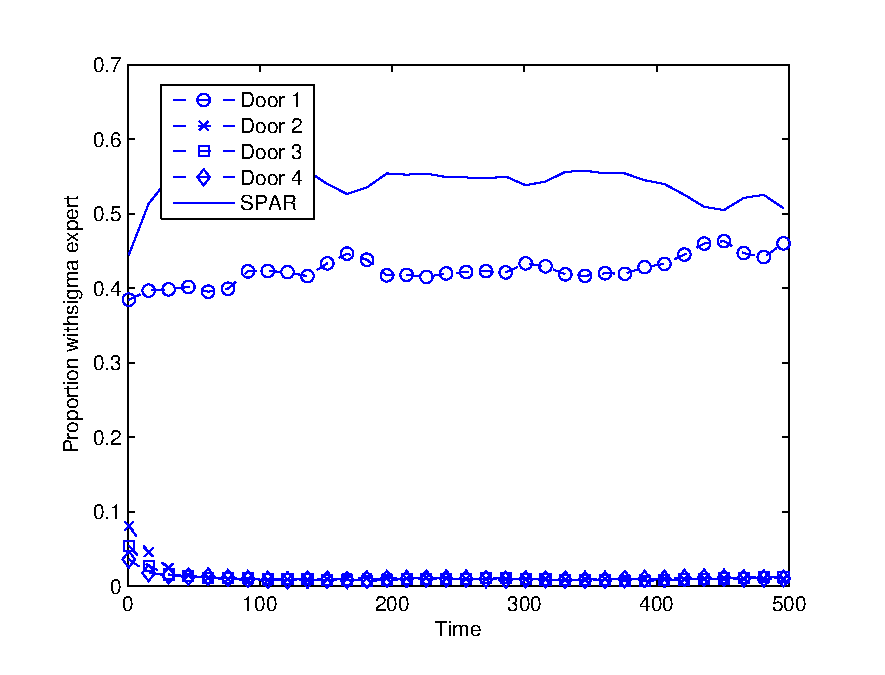
\includegraphics[width=7cm]{img/prob_egreedy_sigma_v4.eps}}
\caption{\label{vs_egreedy_choice}Average proportion of strict
  commands and autonomous SPAR ($\sigma$-policy) decisions vs
  $\epsilon$-greedy User. Costs Setup No4.}
\end{figure}

Our heuristic solution has successfully operated versus the
$\epsilon$-greedy User. Figure~\ref{vs_egreedy} shows smoothed mean
(across interactions sequences) of the SPAR's cost. Graphs show that
the {\em selfish} SPAR inevitably pays greater costs, than the {\em
  User-best} or the {\em $sigma$-policy} SPARs, however the latter two
run at a similar performance level. Essentially, the $\epsilon$-greedy
User was always able to detect the {\em selfish} SPAR, and learn to
avoid its advice. On the other hand, {\em $sigma$-policy} SPAR was
allowed to make an autonomous decision quite often, as can be seen from
Figure~\ref{vs_egreedy_choice} that depicts User choice frequencies
in costs Setup No4.

%% as not detected as explalways explicitly selected
%% the shop to use. This led to higher losses incurred by SPAR. On the
%% other hand, $\sigma$-policy calculated to be fair and honest with
%% respect to the User's utility has received almost complete trust, and
%% was able to utilise the trust to reduce SPAR's costs. As a result, in
%% several setups SPAR's cost is significantly less than that inflicted
%% by the {\em User-best} policy.

\begin{figure}[hbt]
\centerline{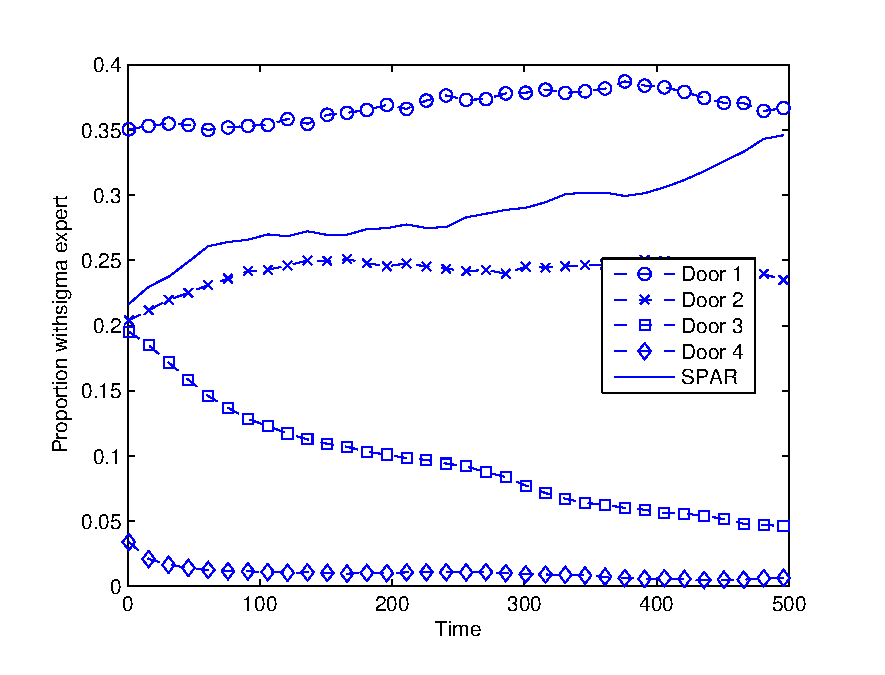
\includegraphics[width=7cm]{img/prob_softmax_sigma_v2.eps}}
\caption{\label{vs_softmax_choice}Average proportion of strict commands and autonomous SPAR decisions vs SoftMax User. Costs Setup No2.}
\end{figure}

\begin{figure*}[ht]
\centerline{\subfigure[Costs Setup No1]{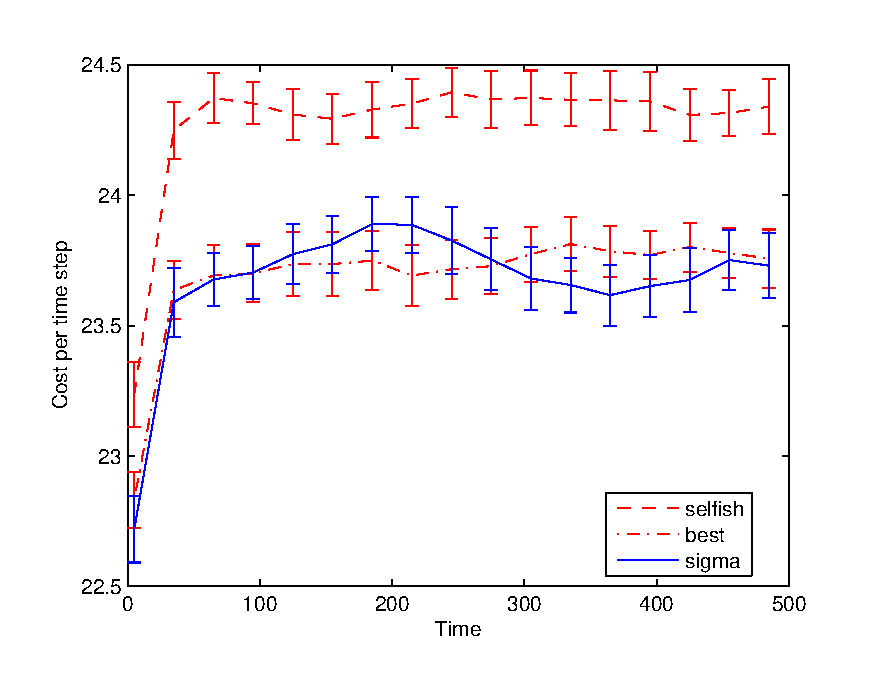
\includegraphics[width=7cm]{img/cost_egreedy_v1.eps}}
\subfigure[Costs Setup No2]{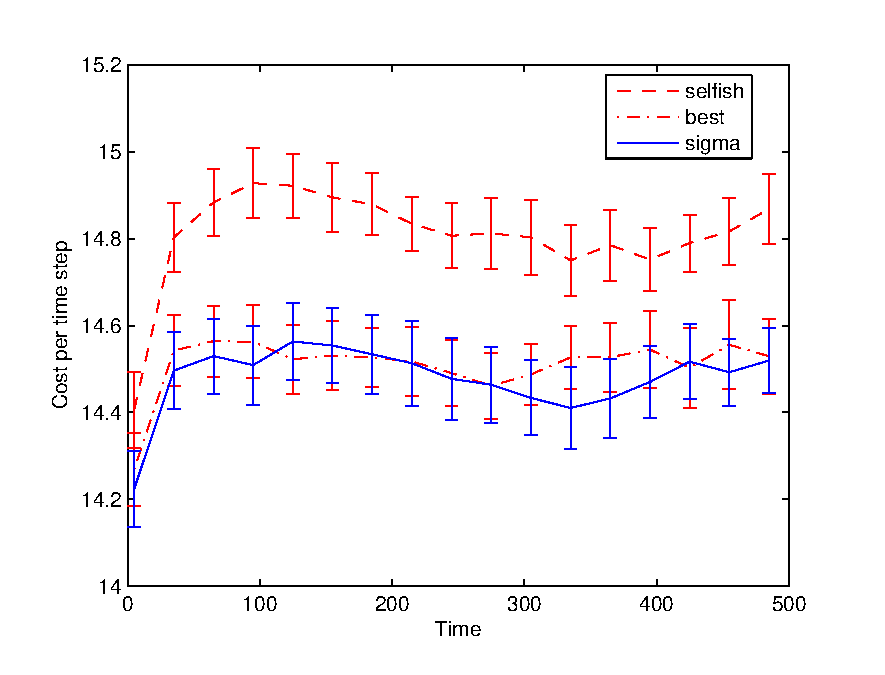
\includegraphics[width=7cm]{img/cost_egreedy_v2.eps}}}
\centerline{\subfigure[Costs Setup No3]{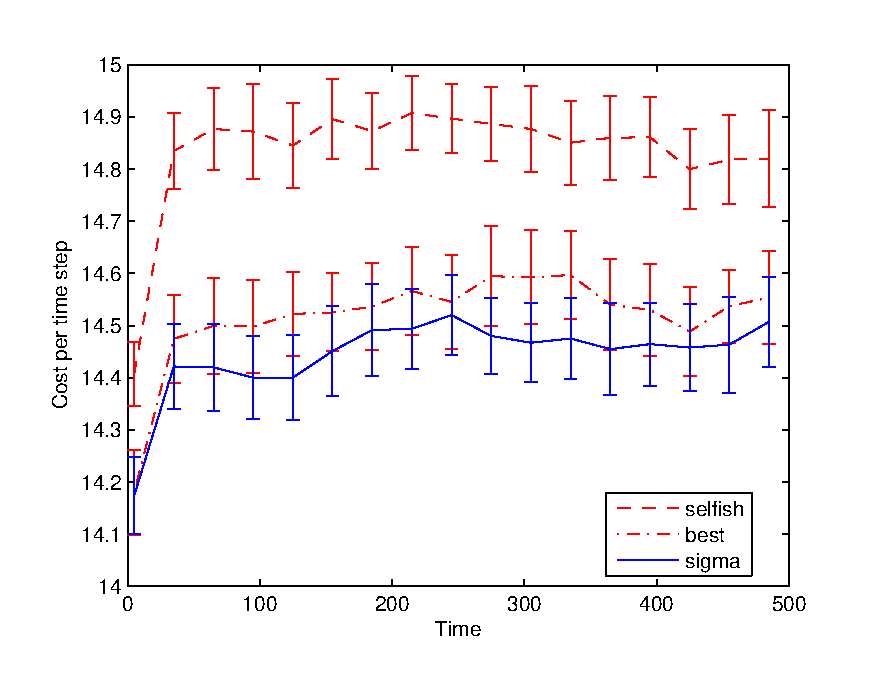
\includegraphics[width=7cm]{img/cost_egreedy_v3.eps}}\subfigure[Costs Setup No4]{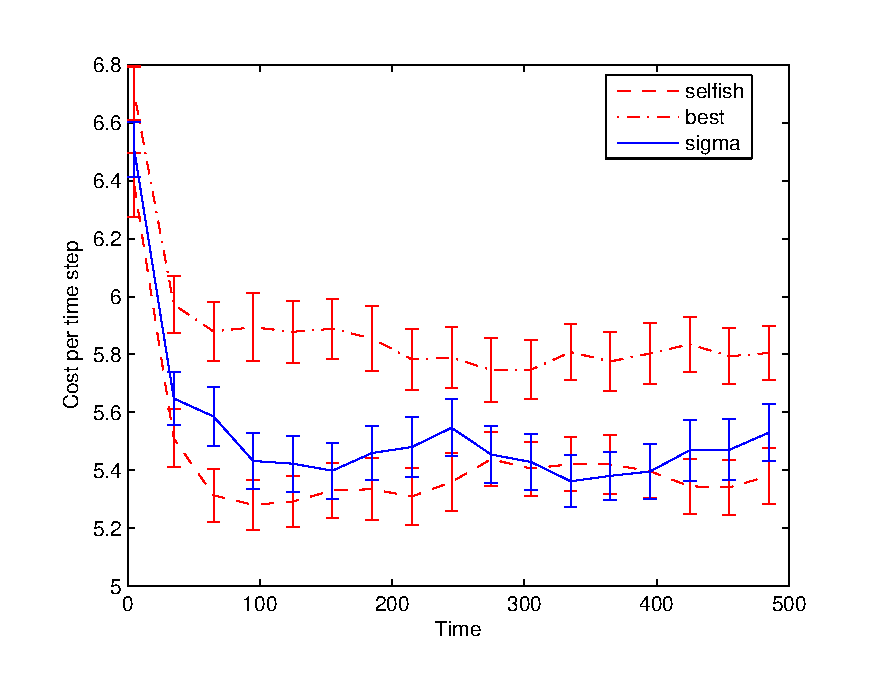
\includegraphics[width=7cm]{img/cost_egreedy_v4.eps}}}
\caption{\label{vs_egreedy} Cost per step vs. $\epsilon$-greedy User.}
\end{figure*}

However, if the User's policy tends to explore and continue to explore
the quality of different services, it becomes much more susceptible to
exploitation by the {\em selfish} SPAR policy. While the exploration
rate of the $\epsilon$-greedy very quickly drops and remains small
($\epsilon$ small, as a matter of fact), the exploration rate of the
SoftMax User depends on the relative difference between the qualities
of services. Unless SoftMax parameter $\tau$ is increased over time or
initially chosen to be very large, SoftMax will continue to switch
between different services, as is demonstrated in
Figure~\ref{vs_softmax_choice}. As a result the {\em selfish} SPAR
policy aggregated the smallest cost among the three SPAR policies vs
the SoftMax User with fixed $\tau$ in all costs Setups (see
Figure~\ref{vs_softmax}). The User continued to allow the {\em
  selfish} SPAR to make an autonomous decision, in spite of its
negative impact on the User's cost.

If, on the other hand, we require that the benevolence of the SPAR
towards User is to be maintained, the $\sigma$-policy becomes the
better choice. In most of our costs Setups the $\sigma$-policy SPAR
significantly outperformed the {\em User-best} SPAR policy. In other
words, while benefiting the User, the $\sigma$-policy SPAR managed to
efficiently control and reduce its own costs. In fact, in several cost
Setups the discrepancy in performance of the $\sigma$-policy and the
{\em selfish} policy diminished over time. For instance in Setup No 1,
the cost aggregated by the {\em selfish} policy grew approaching the
levels of the $\sigma$-policy. At the same time, in the cost Setup No
2 the performance of the $\sigma$-policy approached that of the {\em
  selfish} policy.

%% On the other hand, if the User's policy continued to explore different
%% options much more aggressively, it was susceptible to frequent choices
%% of the shop more beneficial to SPAR than the User. Such was the case
%% with the SoftMax algorithm. The {\em selfish} SPAR policy was quick to
%% exploit these recurrent errors in User's choice, and an equivalent
%% level of cost reduction can not be achieved by an honest
%% SPAR. Nonetheless, it is still possible to reduce the cost in
%% comparison with fully benevolent {\em User-best} SPAR policy, and in
%% several cost setting the discrepancy between $\sigma$-policy and {\em
%%   selfish} policy performance diminished (if not vanished) over
%% time. Figures~\ref{vs_softmax} and ~\ref{vs_softmax_choice} illustrate
%% this situation.

\begin{figure*}[ht]
\centerline{\subfigure[Costs Setup No1]{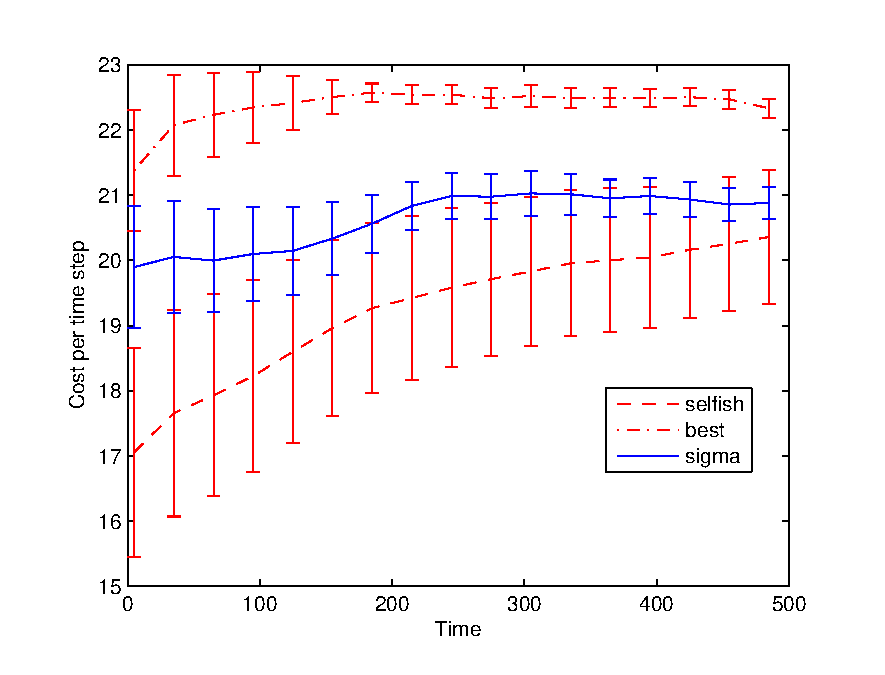
\includegraphics[width=7cm]{img/cost_softmax_v1.eps}}
\subfigure[Costs Setup No2]{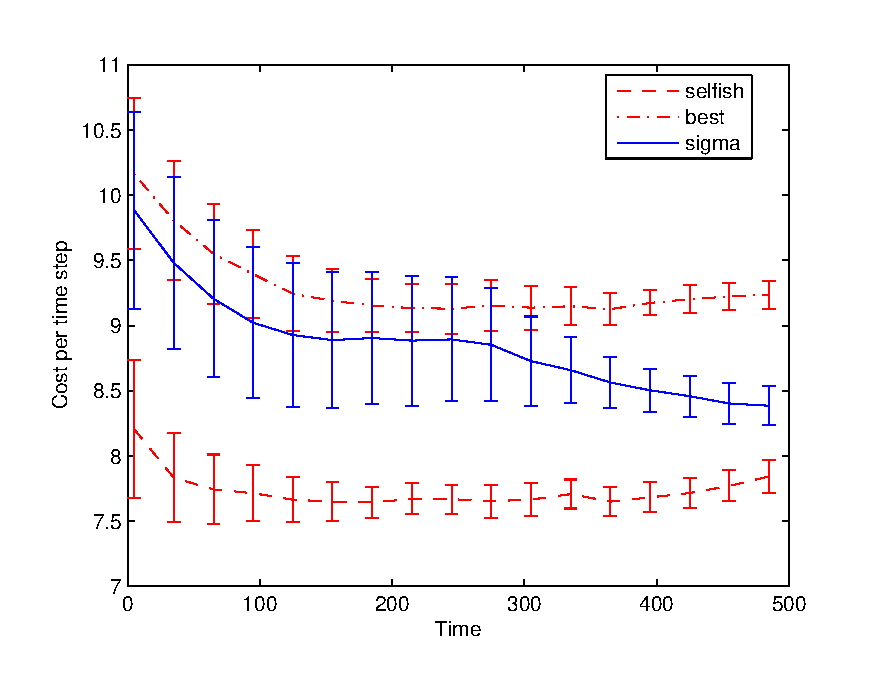
\includegraphics[width=7cm]{img/cost_softmax_v2.eps}}}
\centerline{\subfigure[Costs Setup No3]{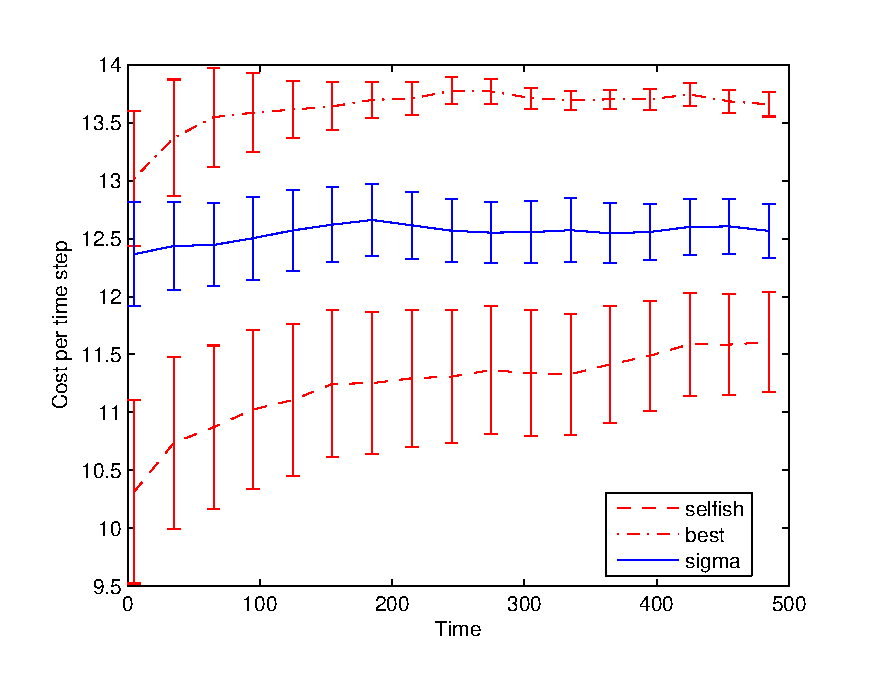
\includegraphics[width=7cm]{img/cost_softmax_v3.eps}}\subfigure[Costs Setup No4]{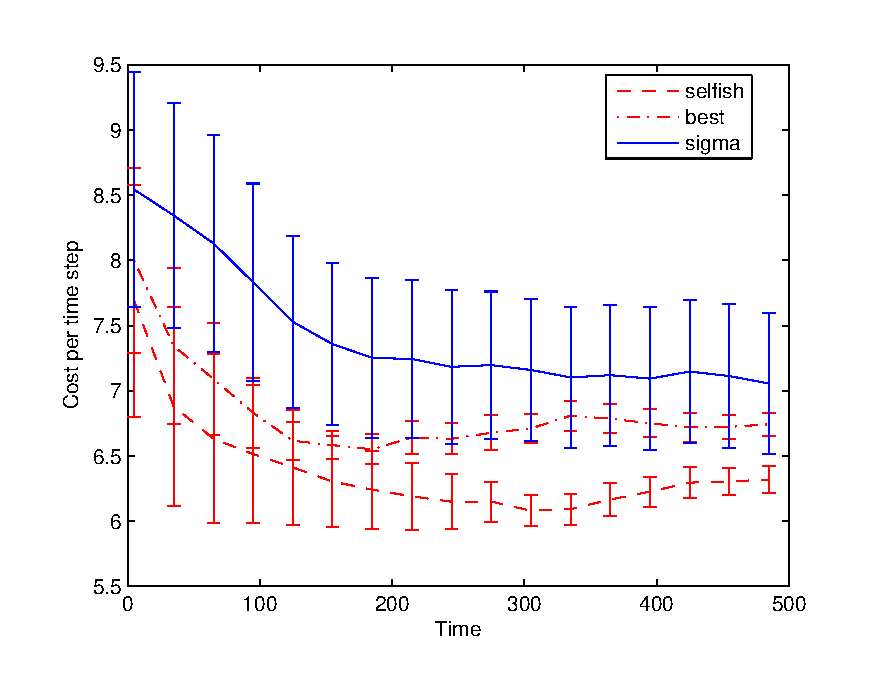
\includegraphics[width=7cm]{img/cost_softmax_v4.eps}}}
\caption{\label{vs_softmax} Cost per step vs. SoftMax User.}
\end{figure*}

\section{Related Work}\label{rel_work}
The {\em Multi-armed bandits (MABs)} have been extensively used before
as the core of an interaction environment model in general, and for
guidance and assistance systems in particular. In the latter case, the
paradigm of environment design or teaching is more commonly adopted
(see e.g.~\cite{Zhang09:General,rdlj_2010_aamas}). Specifically, the
User is assigned the role of MAB's arm selection, while the
guidance/assistance system manipulates the response of different
arms. For example, Chen et al~\cite{chen_etal_2011} investigate the
possibility of off-setting the cost of each arm to induce a particular
pattern in the User's arm choices. However, the possibility to employ
incentives is not universally available in all situations, and other
researchers have preferred User guidance by demonstration. For
instance, Stone et al~\cite{stone_kraus_2010, barrett_stone_2011}
investigate environments where both the User and assistance system
have to pull a MAB's arm, thus forming an ad-hoc team. Allowing for
even less involvement, ~\cite{arkgg_2012} investigate the case where
the system merely suggests a choice to the User. Notice, however, that
none of these models can be directly applied to the interaction
characteristic of our 4-door game example, since they do not address
the User's delegation of the arm choice to the assistance system,
where the system first performs an action and only reports on
it. Interestingly enough, the opposite situation has been
investigated. For example, Sofman et
al. ~\cite{sofman_bagnell_stentz_2009} discuss a model where the human
User is viewed as an arm in a MABs and it is the system that chooses
an arm. In their paper, the model captures the situation where the
assistant system needs to decide when (if at all) to relinquish its
autonomy and delegate the task back to the User.

\section{Conclusions}\label{conclusions}

In this paper we have introduced a new type of interaction between an
adaptive User and a self-preserving assistant robot (SPAR). The
interaction allows the SPAR to have action costs different from those
of the User, but limits the SPAR's autonomy. In more detail, the User
chooses between explicitly instructing the SPAR to perform a specific
action, or allows the SPAR to make the decision autonomously. Due to
SPAR's desire to reduce its own costs, during autonomous choices it
can choose an action sub-optimal from the User's point of view. This,
however, has to be balanced with gaining User's trust. Otherwise the
User will never allow the SPAR to make the choice autonomously. To
achieve this balance, we fully formalise the problem by: a) modelling
the User as a Multi-Armed Bandit solution algorithm; b) modelling the
SPAR's decision problem as an expected average cost Markov decision
problem; c) we explicitly limit the SPAR to benevolent solutions,
that guarantee not to increase the User's costs.

In addition, this paper provides an approximation algorithm for the
SPAR's MDP problem, based on unscented filter method and a heuristic
stabilisation meta policy -- $\sigma$-heuristic. We experimentally
show that the approximation performs correctly with respect to 
benevolence towards the User, and reduces SPAR's costs where possible under
this constraint.

As a future work we plan to investigate performance of
$\sigma$-heuristic against models of human behaviour, as well attempt
an analytical solution of SPAR's EAC-MDP.

\bibliography{ecai2012}
\end{document}

